\begin{frame}{Simplification}
	\begin{itemize}
		\item Construct a quad tree
			\only<1> {
				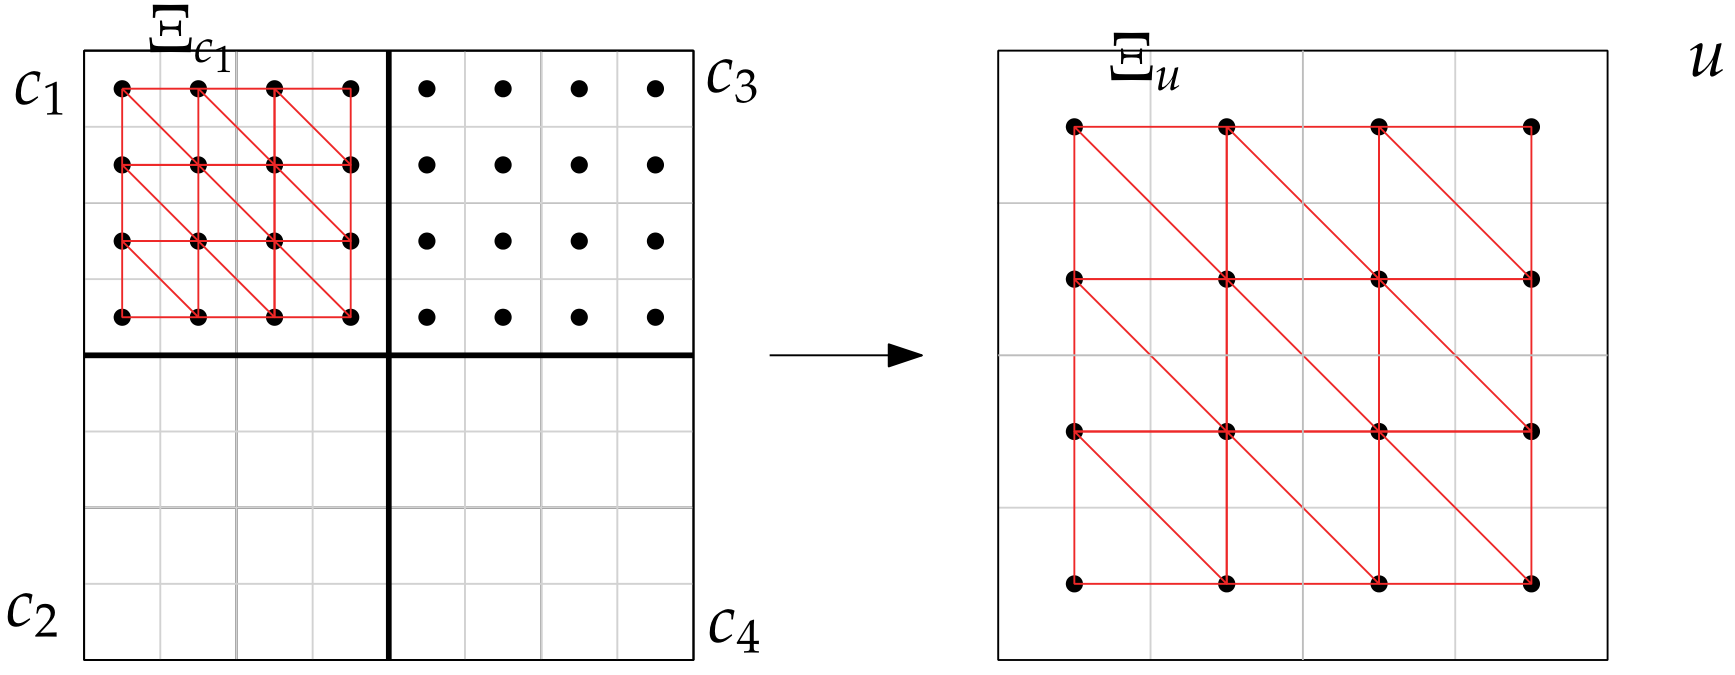
\includegraphics[height=0.5\textheight]{algorithm-simplification-gridconstruction}
			}
		\item Approximate terrain surface
			\only<2> {
				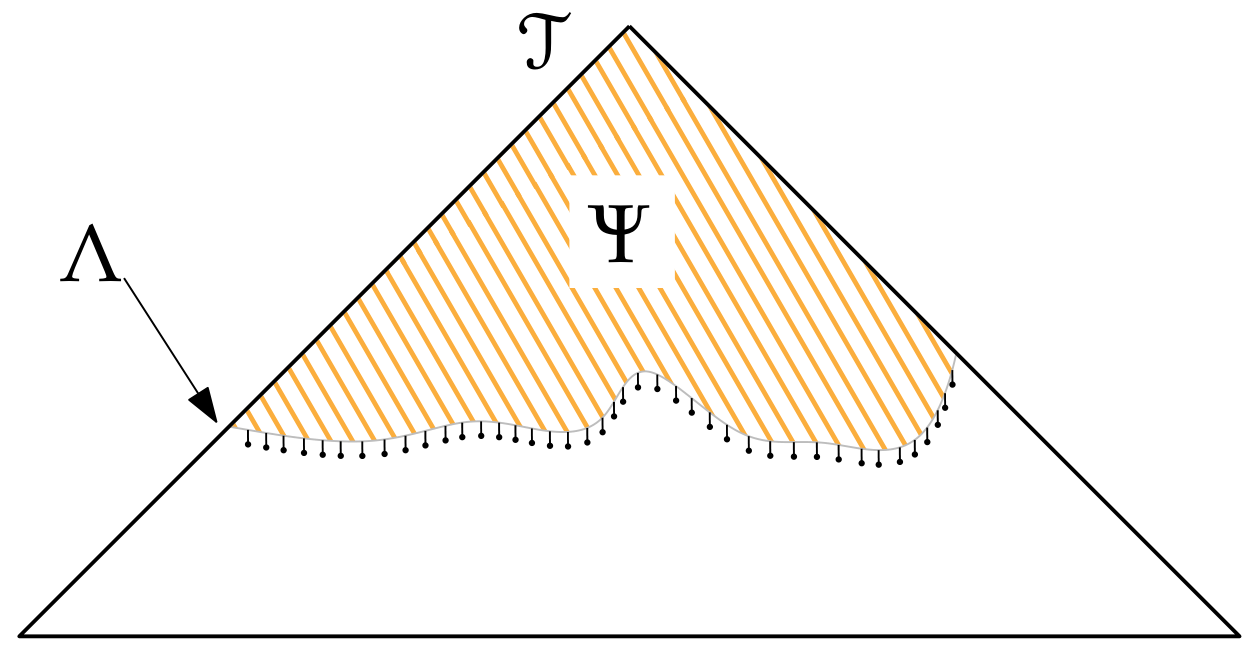
\includegraphics[height=0.5\textheight]{algorithm-simplification-quadtree}
			}
			\only<3> {
				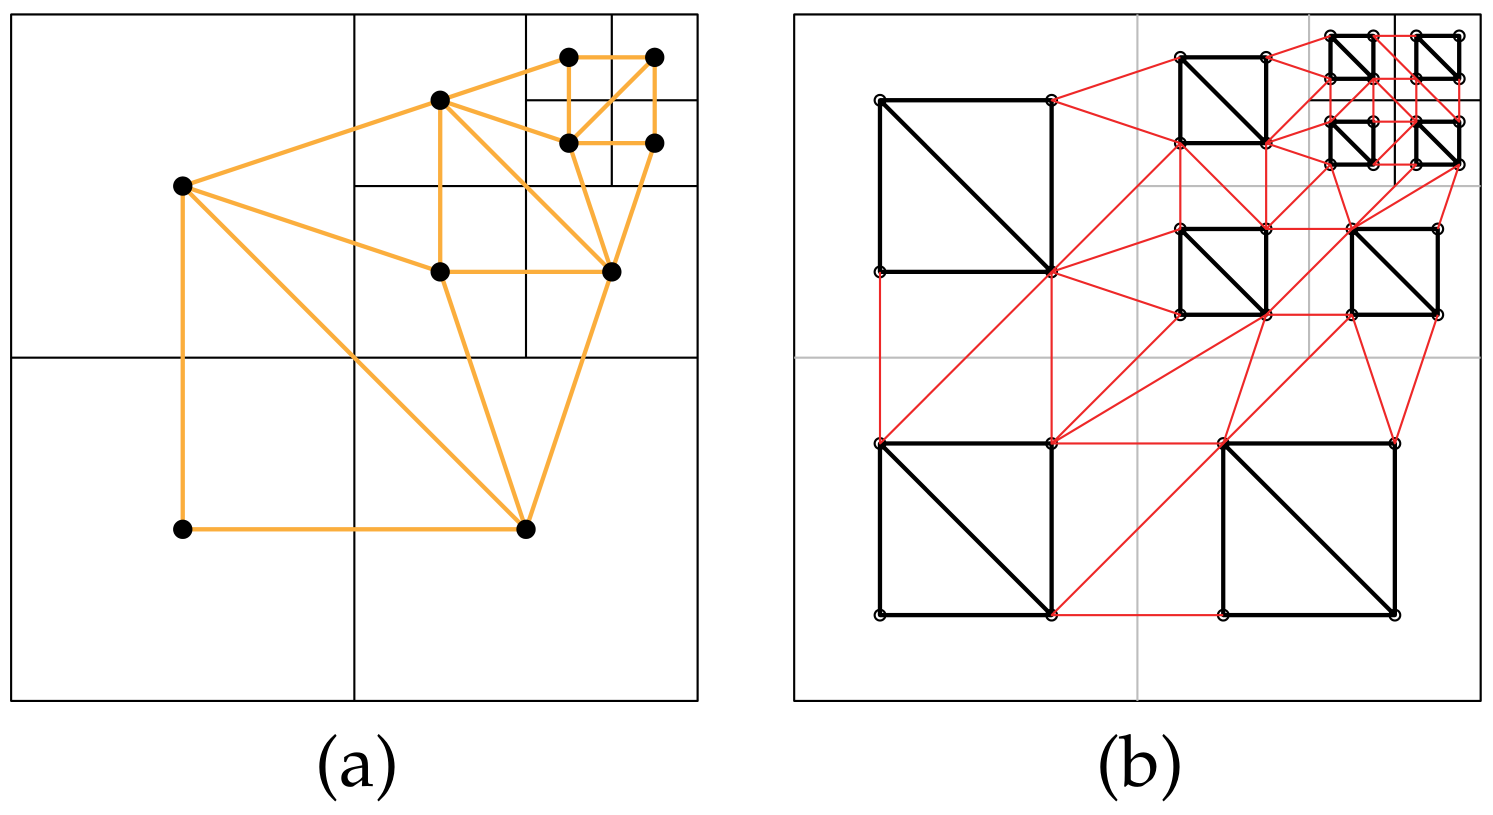
\includegraphics[height=0.5\textheight]{algorithm-simplification-dual}
			}
		%TODO: Notes on how this works
	\end{itemize}
\end{frame}

\begin{frame}{Example}
	\centering
	\only<1>{\exampleimg{grid}}%
	\only<2>{\exampleimg{grid-0}}%
	\only<3>{\exampleimg{grid-1}}%
	\only<4>{\exampleimg{grid-2}}%
	\only<5>{\exampleimg{grid-3}}%
	\only<6>{\exampleimg{grid-4}}%
	\only<7>{\exampleimg{grid-5}}%
\end{frame}

\begin{frame}{Computing the map}
	\begin{itemize}
		\item Compute the visibility map restricted to part of the tree
			\only<1> {
				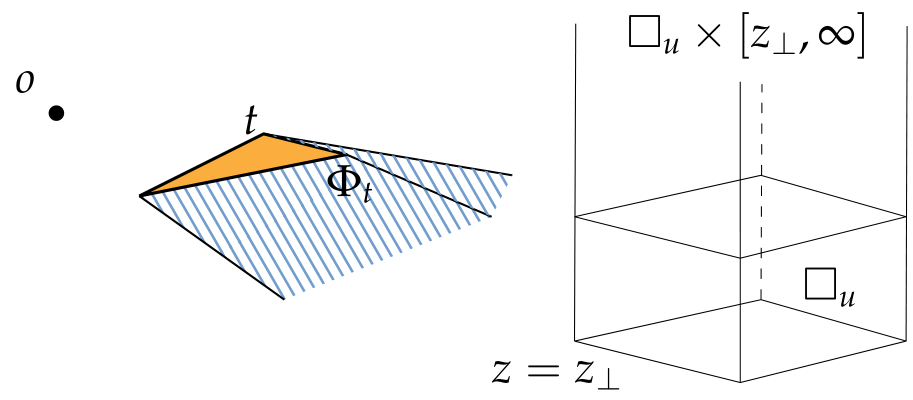
\includegraphics[height=0.5\textheight]{algorithm-map-shadow}
			}
		\item Compute the occluder set
		\item approximate $\tilde{V}_u$
		\note{
			The squares that can throw a shadow are the shadow frustrum
		}
	\end{itemize}
\end{frame}

\begin{frame}{Using the GPU}
	\begin{itemize}
		\item GPU is useful for doing many simple calculations
		\item Cast rays from observers to square
		\item Read out color buffer
	\end{itemize}
\end{frame}
